\documentclass[12pt, twoside]{article}
\usepackage[letterpaper, margin=1in, headsep=0.5in]{geometry}
\usepackage[english]{babel}
\usepackage[utf8]{inputenc}
\usepackage{amsmath}
\usepackage{amsfonts}
\usepackage{amssymb}
\usepackage{tikz}
\usetikzlibrary{quotes, angles}
\usepackage{graphicx}
\usepackage{enumitem}
\usepackage{multicol}

\newif\ifmeta
\metatrue %print standards and topics tags

\title{Regents Geometry}
\author{Chris Huson}
\date{September 2020}

\usepackage{fancyhdr}
\pagestyle{fancy}
\fancyhf{}
\renewcommand{\headrulewidth}{0pt} % disable the underline of the header
\raggedbottom


\fancyhead[LE]{\thepage}
\fancyhead[RO]{\thepage \\ Name: \hspace{4cm} \,\\}
\fancyhead[LO]{BECA / Dr. Huson / Geometry \\* 1-3 Mastery assessment (Open book)}

\begin{document}

\subsubsection*{I can solve for segment lengths}
\begin{enumerate}
\item Given $\overline{ABC}$, $AB=8$, and $BC=4$. Find ${AC}$.\\[1cm]
    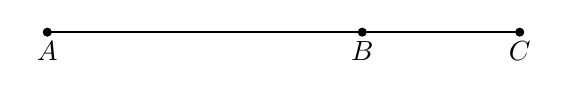
\begin{tikzpicture}
      \draw [-, thick] (0,0)--(6,0);
      \draw [fill] (0,0) circle [radius=0.05] node[below]{$A$};
      \draw [fill] (4,0) circle [radius=0.05] node[below]{$B$};
      \draw [fill] (6,0) circle [radius=0.05] node[below]{$C$};
    \end{tikzpicture} \vspace{1cm}
    
\item Given $\overline{RST}$, $RS=5$, and $RT=7 \frac{1}{2}$.
  \begin{enumerate}
  \item Find ${ST}$.\\[0.75cm]
    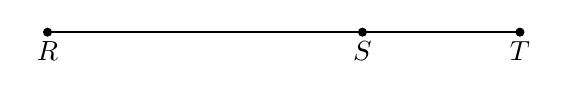
\begin{tikzpicture}
      \draw [-, thick] (1,0)--(7,0);
      \draw [fill] (1,0) circle [radius=0.05] node[below]{$R$};
      \draw [fill] (5,0) circle [radius=0.05] node[below]{$S$};
      \draw [fill] (7,0) circle [radius=0.05] node[below]{$T$};
    \end{tikzpicture}  \vspace{1cm}
  \item The postulate used in this problem is the \rule{6cm}{0.15mm}.
  \end{enumerate} \vspace{0.5cm}

\item Given $\overline{DEF}$, $DE=x+4$, $EF=x+2$, $DF=14$. Find ${DE}$.
  \begin{enumerate}
  \item Label the diagram with the given values.
  \begin{flushright}
    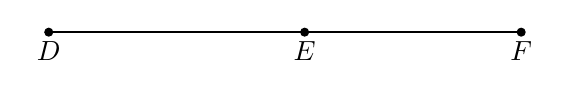
\begin{tikzpicture}
        \draw [-, thick] (0,0)--(6,0);
        \draw [fill] (0,0) circle [radius=0.05] node[below]{$D$};
        \draw [fill] (3.25,0) circle [radius=0.05] node[below]{$E$};
        \draw [fill] (6,0) circle [radius=0.05] node[below]{$F$};
    \end{tikzpicture}
  \end{flushright} \vspace{0.5cm}
  \item Write an equation: \vspace{1cm}
  \item Solve for $x$
  \vspace{3cm}
  \item Answer the question. \\
  Find $DE$ by substituting for $x$. \vspace{1.5cm}
  \item Check your answer
  \end{enumerate}
  %\vspace{2cm}

\newpage
\item Early finishers: In the following two problems, solve for the value of $x$.
  \begin{multicols}{2}
    \begin{enumerate}
      \item   $3x-3=x + 7$ \vspace{6cm}
      \item   $\frac{1}{2}(4x+2)=7$ \vspace{6cm}
    \end{enumerate}
  \end{multicols}
  \vspace{5cm}

\item Given the linear function $f(x)=2x-6$.
\begin{multicols}{2}
  \begin{enumerate}
    \item   $f(x)=0$. Find $x$. \vspace{6cm}
    \item Find $f(2)$ \vspace{6cm}
  \end{enumerate}
\end{multicols}
  \vspace{6cm}

\item Given $x^2+8x+7=0$. Factor and find the roots. \vspace{4cm}

\end{enumerate}
\end{document}